\chapter{実験方法}\label{EM}

CheCoProの協調プログラミング支援効果の検証を目的に実験を行った.初学者の協調プログラミングにおけるインタラクションのパターンの抽出と,アンケートによる協調プログラミングの意識調査を行った.

%----------6.1--------
\section{学習環境と課題内容}

2014年度秋学期に開講された静岡大学のプログラミング入門講義において実験を行った.プログラミング入門講義は,週2コマの必修の授業である.受講者は,情報学部情報社会学科(文科系)1年生である.実験を行うまでに,受講者はオブジェクト指向の概念を除くJavaの基礎的な学習に4ヶ月間取り組んでいる.協調プログラミングに取り組むことは未経験である.


\begin{table}[tb] 
\caption{課題内容} 
\label{tab:final}
\hbox to\hsize{\hfil
\begin{tabular}{l|ll}\hline\hline
課題		& Javaを使ったGUI作品制作 \\
期間		& 2週間 \\
グループ人数 	& 1〜3名 \\
構成メンバ	& 受講生同士で任意に決定 \\\hline
\end{tabular}\hfil}
\end{table}


実験は,当該講義の最終課題として行った.最終課題の要項を\tabref{tab:final}に示す.最終課題の内容は,Javaを用いたGUI作品の制作である.課題に取り組む期間は2週間である.グループは上限3名であり,メンバは受講者が任意で決めたものである.


%----------6.2--------
\section{システムの導入と利用群,非利用群のグループ分け}

まず,最終課題にエントリした全44組(104名)から,1人グループ8組を除いた36組(96名)を分析対象とした.

CheCoProの導入方法と機能に関する説明を行った上で,CheCoProを利用するかどうかは任意とし,最終的にそのグループの利用状況で利用群と非利用群を分けた.その結果を\tabref{tab:record}に示す.
利用群は15組(3人グループ8組,2人グループ7組),非利用群は21組(3人グループ16組,2人グループ5組)であった.

\begin{table}[tb] 
\caption{グループの内訳と成績} 
\label{tab:record}
\hbox to\hsize{\hfil
\begin{tabular}{c|cc}\hline\hline
				& 利用群 	& 非利用群 \\\hline
組数(割合)		& 15組(41.7\%)	& 21組(58.3\%)\\
成績の平均\footnotemark[2] 	& 51.2 (sd=7.38) 	& 49.4 (sd=8.99) \\\hline
\end{tabular}\hfil}
\end{table}


\footnotetext[2]{この時点までに取得できる成績の最高点は73である} 

この時,CheCoProの導入方法と機能に関する説明は,被験者全員に対して行った(約10分)その後,全グループに対して,CheCoProがすぐに使えるよう初期設定を行った.このようにして,初期設定の煩わしさを理由としてCheCoPro非利用を学習者が選択することを避けた.

この方式での利用,非利用群の分離は,学習者が学習の状況を考えて環境を学習者自身が選択できる反面,利用群と非利用群にプログラミングの能力差が出る可能性がある.そこで,各群のプログラミング能力が概ね等質であることを調べるために,各群の成績の差を調べた.\tabref{tab:record}に示された成績は最終課題に入る前までの講義の成績であり,課題の提出状況と提出物の内容から,講義担当者と著者を含むティーチングアシスタントによって確定したものである.利用群の平均は51.2(sd=7.38),非利用群の平均は49.4(sd=8.99)であった.t検定(以下,断りのない限りWelchの法による)を行った結果,平均の差は有意でなかった(両側検定:t(89.0)=1.10,n.s.).以上より,両群のプログラミング能力について同等であることを確認した.

%----------6.3--------
\section{分析方法}

%----------6.3.1------
\subsection{アンケート}

協調プログラミングに対するフォロワの意識調査から,独立同期モデルの有効性を検証するために,アンケート結果の分析を行った.

アンケート項目の中で,協調プログラミングの達成に重要と考えられる「遠慮」と「貢献」について尋ねたアンケート結果に関して分析を行った.協調プログラミング中の遠慮と貢献の度合いを,「強くそう思う」「そう思う」「そう思わない」「強くそう思わない」の4段階のリッカート尺度を用いて自己評価を行うアンケート項目である.

フォロワの意識の変化が協調プログラミングの成功に繋がると考えられるため,成績の順位を用いて,グループ内のでの順位が1位の者以外をフォロワとして抽出した.ドライバはコーディングにおいてプロジェクトに最も主体的に参加しているメンバと定義したとおり,プロジェクトに積極的に貢献していることが前提である.しかし,フォロワの貢献度合いに関してはグループごとによって異なっていた.


%----------6.3.2------
\subsection{インタラクションパターン}


\begin{figure}[tb]
	\begin{center}
		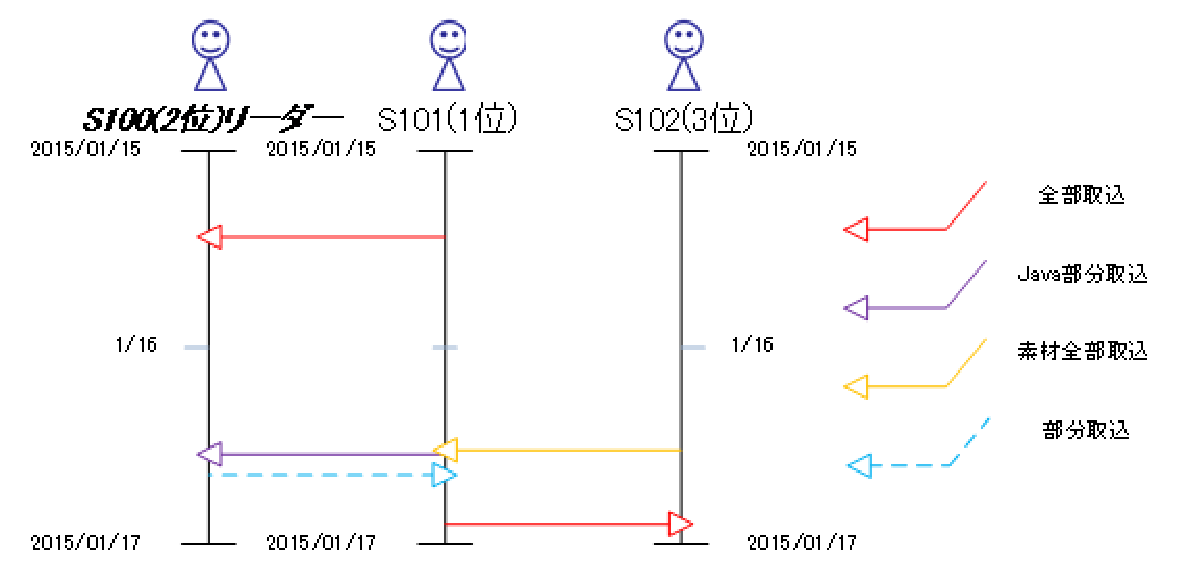
\includegraphics[width=\linewidth]{img/flowSample.eps}
		\caption{インタラクション図(例)}
		\label{fig:flowSample}
	\end{center}
\end{figure}


プログラミング初学者の協調プログラミングの実態解明を目的に,インタラクション図の作成と質的分析による評価を行った.

インタラクション図とは,グループメンバ同士の取り込みのやりとりを時系列に表した図である.インタラクション図の例を\figref{fig:flowSample}に示す.縦軸は時間を表す.それぞれの軸の上に記述されている番号はメンバのIDであり,括弧内の数字はグループ内での成績の順位を表す.グループのリーダ\footnotemark[3] は左端に配置し,その他のメンバは左から成績の高い順に配置した.各矢印は取り込みを表し,矢印先のメンバが矢印元のメンバのソースコード等を取り込んだことを表す.

\footnotetext[3]{グループのリーダはグループメンバ同士で任意に決めたものである}

インタラクション図は利用群全15グループに対して作成した.インタラクション図に対する質的な分析から典型的なインタラクションのパターンを抽出することを試みた.

インタラクション図は,ファイルやソースコードの取り込みを表す図である.したがって,被験者がどのような意図で取り込みを行ったのかは把握できない.被験者の行動の意図については,取り込みを行った日時,頻度,ファイルの種類等,インタラクション図の文脈からの推測となる.しかし,推測は被験者に対するインタビューの経験2例から概ね正確であることがわかっている\cite{加藤優哉2014}.


%----------6.3.3------
\subsection{インタラクションと成績}

グループ内のプログラミング能力の差とインタラクションの関係性を調査するために,同講義の成績を用いて分析を行った.本分析では,collective contributionにおけるCheCoProの有効性の検証を試みた.

成績がドライバに近いフォロワはソースコードの提供による貢献をし,ドライバよりも著しく成績が低いフォロワはテストによる貢献にとどまると考えられる.従って,フォロワについて,ソースコードの提供による貢献かテストによる貢献のいずれか一方での貢献に偏っていることが顕著に現れているグループのインタラクション図を抽出した.抽出したグループに関して各メンバの成績と照らし合わせることによって分析を進めた.